% Anhang content
%
\chapter{Project Plan} \label{app:ProjectPlan}
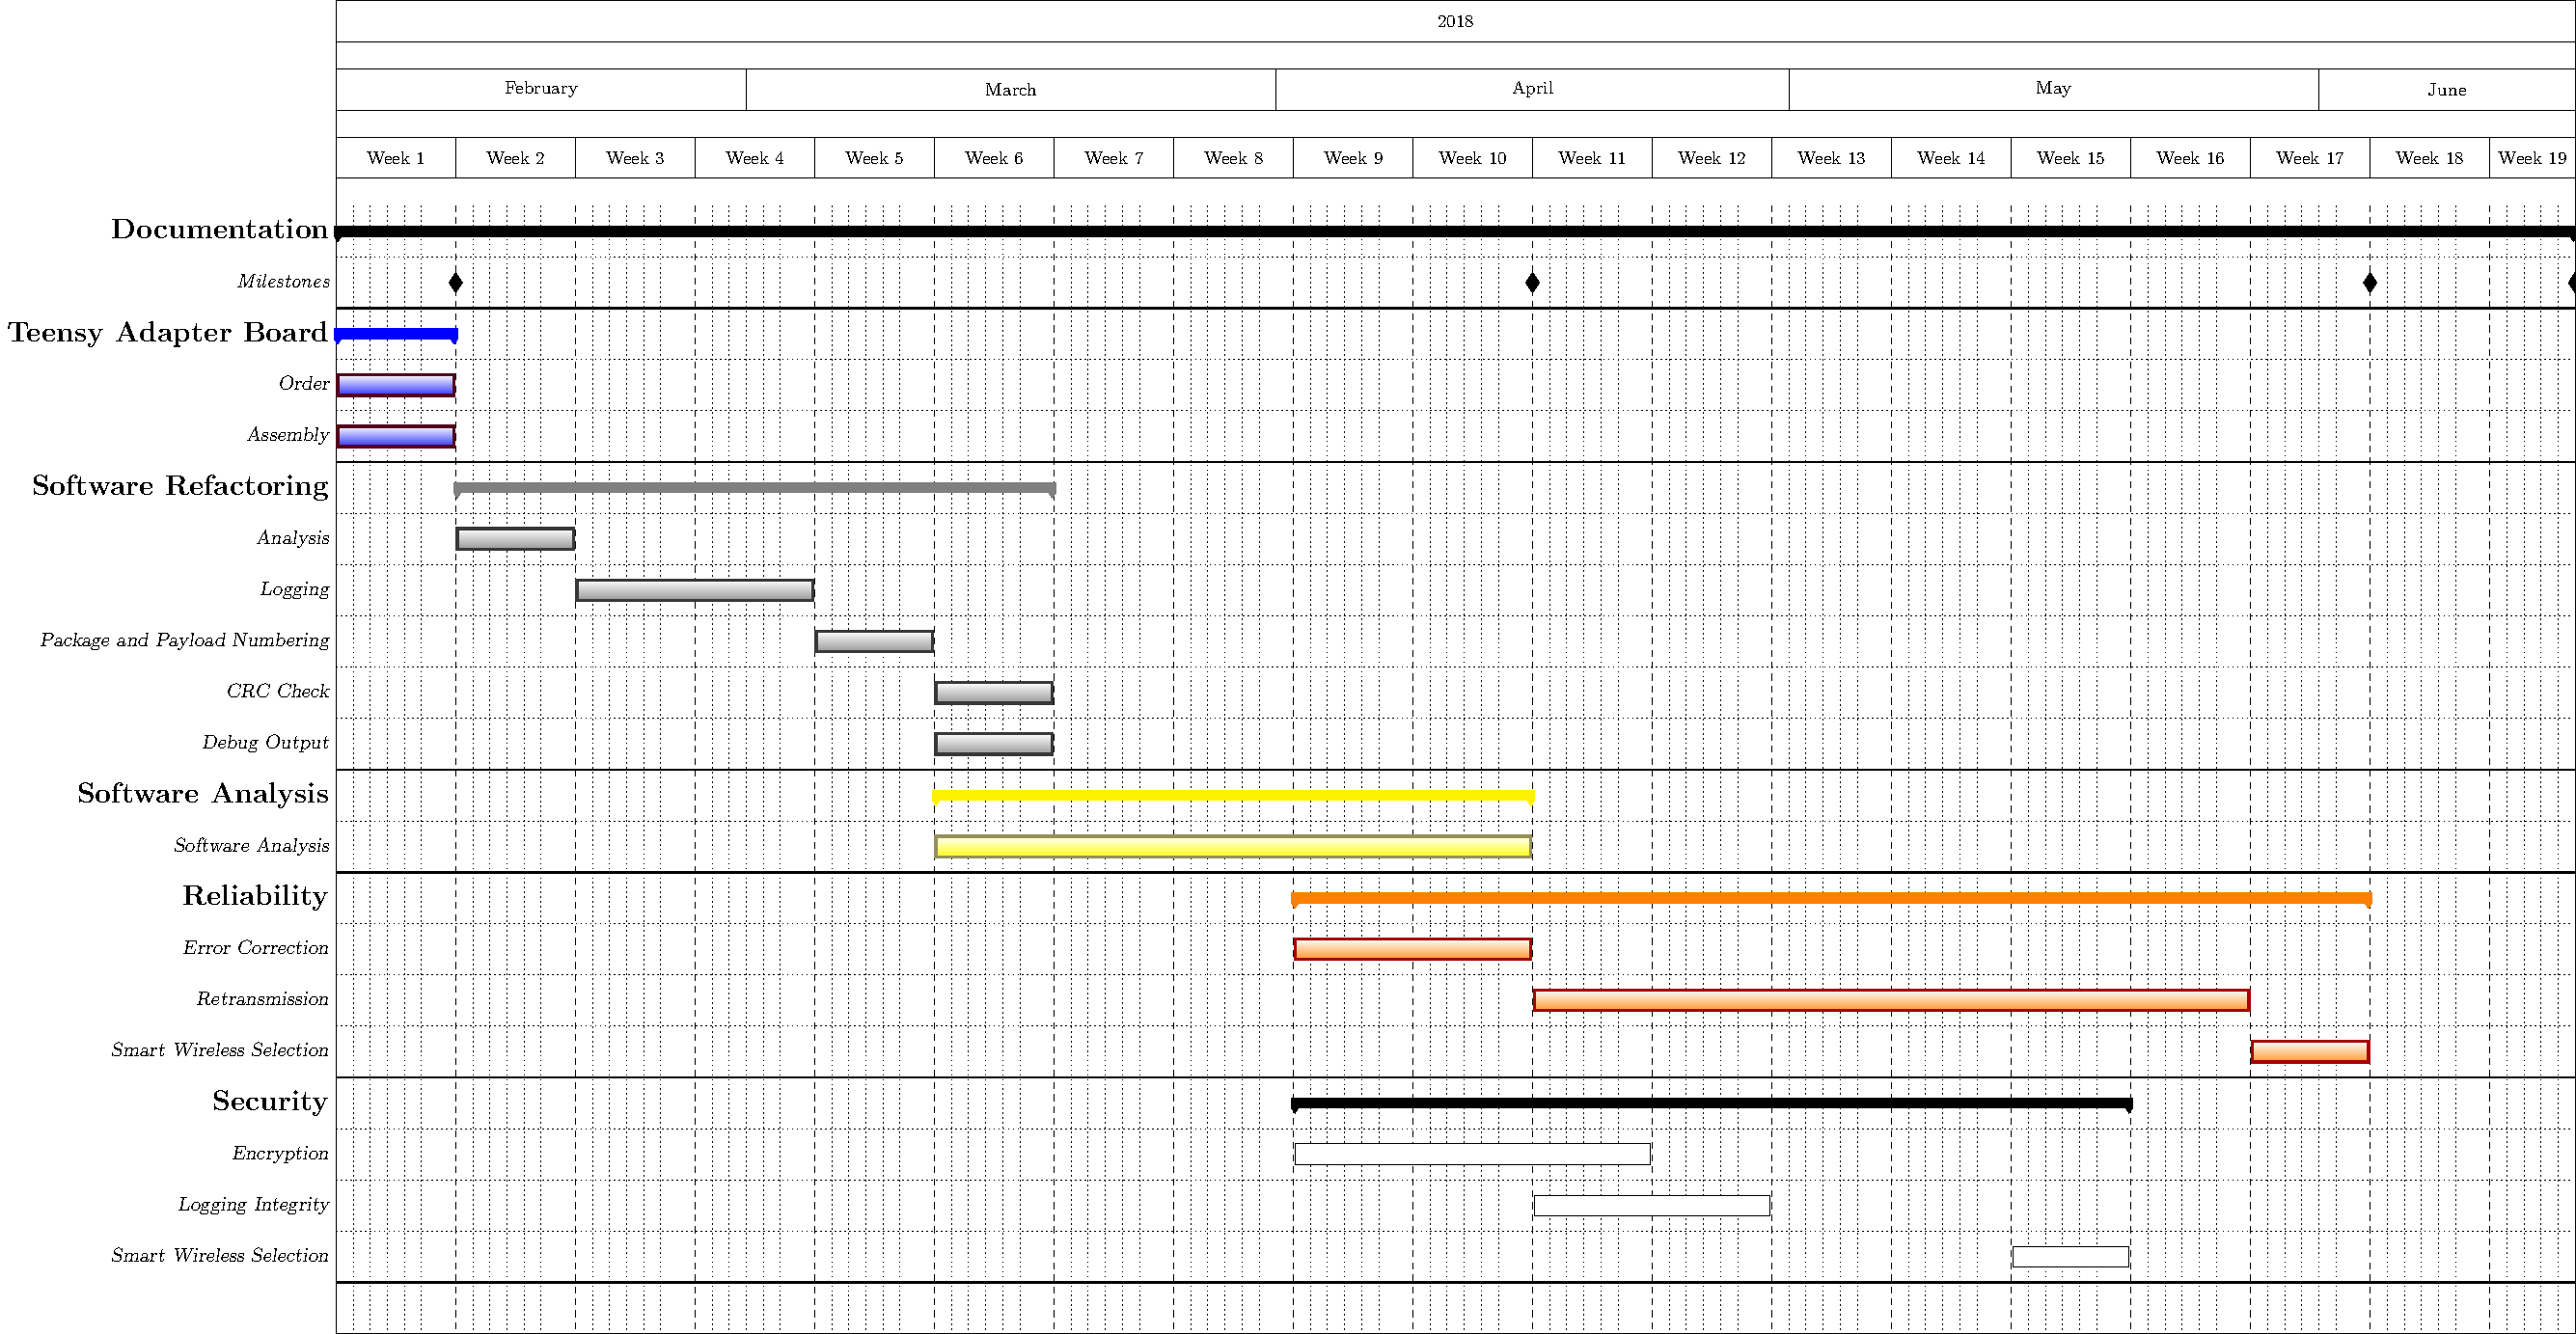
\includepdf[pages=-, angle=90, scale=0.9]{ProjectPlan.pdf}
%
%
%
%
%
%
\chapter{Configuration File}\label{app:txtConfigFile}
A sample configuration file as saved on the SD card looks as follows:
\begin{lstlisting}
;=====================================================================================
[BaudRateConfiguration]
;
;
; BAUD_RATES_WIRELESS_CONN
; Configuration of baud rates on wireless side from 0 to 3.
; Regarding the supported baud rates see implementation of hwBufIfConfigureBaudRate in hwBufferInterface.cpp
BAUD_RATES_WIRELESS_CONN = 57600, 57600, 57600, 57600
;
;
; BAUD_RATES_DEVICE_CONN
; Configuration of baud rates on wireless side from 0 to 3.
; Regarding the supported baud rates see implementation of hwBufIfConfigureBaudRate in hwBufferInterface.cpp
BAUD_RATES_DEVICE_CONN = 57600, 57600, 38400, 38400
;
;
;=====================================================================================
[ConnectionConfiguration]
;
;
; PRIO_WIRELESS_CONN_DEV_X
; Priority of the different wireless connections from the viewpoint of a single device.
; 0: Wireless connection is not used; 1: Highes priority; 2: Second priority, ..
PRIO_WIRELESS_CONN_DEV_0 = 1, 1, 0, 0
PRIO_WIRELESS_CONN_DEV_1 = 1, 1, 0, 0
PRIO_WIRELESS_CONN_DEV_2 = 0, 0, 1, 0
PRIO_WIRELESS_CONN_DEV_3 = 0, 0, 0, 1
;
;
; SEND_CNT_WIRELESS_CONN_DEV_X
; Number of times a package should be tried to be sent over a single wireless connection.
SEND_CNT_WIRELESS_CONN_DEV_0 = 1, 0, 0, 0
SEND_CNT_WIRELESS_CONN_DEV_1 = 0, 1, 0, 0
SEND_CNT_WIRELESS_CONN_DEV_2 = 0, 0, 1, 0
SEND_CNT_WIRELESS_CONN_DEV_3 = 0, 0, 0, 1
;
;
;=====================================================================================
[TransmissionConfiguration]
;
;
; RESEND_DELAY_WIRELESS_CONN
; Time in ms that should be waited until a package is sent again when no acknowledge is received per wireless connection.
RESEND_DELAY_WIRELESS_CONN = 255, 255, 255, 255
;
;
; MAX_THROUGHPUT_WIRELESS_CONN
; Maximal throughput per wireless connection (0 to 3) in bytes/s.
MAX_THROUGHPUT_WIRELESS_CONN	 = 10000, 10000, 10000, 10000
;
;
; USUAL_PACKET_SIZE_DEVICE_CONN
; Usual packet size per device in bytes if known or 0 if unknown.
USUAL_PACKET_SIZE_DEVICE_CONN	= 50, 50, 1, 1
;
;
; PACKAGE_GEN_MAX_TIMEOUT
; Maximal time in ms that is waited until packet size is reached. If timeout is reached, the packet will be sent anyway, independent of the amount of the available data.
PACKAGE_GEN_MAX_TIMEOUT	= 20, 20, 20, 20
;
;
; DELAY_DISMISS_OLD_PACK_PER_DEV
DELAY_DISMISS_OLD_PACK_PER_DEV	= 10000, 10000, 10000, 10000
;
;
; SEND_ACK_PER_WIRELESS_CONN
; To be able to configure on which wireless connections acknowledges should be sent if a data package has been received. Set to 0 if no acknowledge should be sent, 1 if yes.
SEND_ACK_PER_WIRELESS_CONN	= 0, 0, 0, 0
;
;
; USE_CTS_PER_WIRELESS_CONN
; To be able to configure on which wireless connections CTS for hardware flow control should be used. Set to 0 if it shouldn't be used, 1 if yes.
; If enabled, data transmission is stopped CTS input is high and continued if low.
USE_CTS_PER_WIRELESS_CONN	= 0, 0, 0, 0
;
;
; PAYLOAD_REORDERING_TIMEOUT
; When the package numbering processing mode is set to 3, this timeout will configure, how long the program waits for the correct next
; package to arrive before sending the data out anyway (even with one package missing in the middle)
PAYLOAD_REORDERING_TIMEOUT		= 100, 100, 100, 100
;
;
; PAYLOAD_NUMBERING_PROCESSING_MODE
; Received packages can be processed in 3 ways:
; 		1	The payload number is ignored and received packages are sent out on device side in the same order as the were received on wireless side
;		2	The received packages are put into order again with the use of an internal array
;		3	Only the newest packages are processed
; This parameter is per device side
PAYLOAD_NUMBERING_PROCESSING_MODE	= 3, 1, 1, 1
;
;
; SYNC_MESSAGING_MODE_ENABLED_PER_WL_CONN
; This mode can be enabled per wireless connection. If enabled (=1), then the next package is only sent when the last one was received successfullly
SYNC_MESSAGING_MODE_ENABLED_PER_WL_CONN	= 0, 0, 0, 0
;
;
; LOAD_BALANCING_MODE
; This mode determines how a wireless connection for (re-)send attempts is chosen.
;		1	(Re)sending is done according to this config file, first x attempts on prio 1 and, y attempts on prio 2 etc
;		2	(Re)sending is done according to received acknowledges. Once an acknowledge is not received, the next send attempts will be done with an other wl conn
;		3	(Re)sending is done according to an algorithm that takes various aspects into account.
LOAD_BALANCING_MODE = 1
;
; USE_GOLAY_ERROR_CORRECTING_CODE
; Golay can correct up to xx bitflips, configuration per wireless side
USE_GOLAY_ERROR_CORRECTING_CODE = 0, 0, 0, 0
;=====================================================================================
[SoftwareConfiguration]
;
;
; TEST_HW_LOOPBACK_ONLY
; Set to 0 for normal operation, 1 in order to enable loopback on all serial interfaces in order to test the hardware.
TEST_HW_LOOPBACK_ONLY	= 0
;
; ENABLE_STRESS_TEST
; Instead of reading bytes from device side, 10 bytes of data will be pushed onto the device RX queue on every SPI_HANDLER_TASK_INTERVAL
ENABLE_STRESS_TEST= 0
;
; GENERATE_DEBUG_OUTPUT
; The amount of debug output on the RTT Shell can be configured in three ways:
;		1	No debug output, RTT disabled, shell not configured
;		2	Only the shell is running, commands are parsed, no SW specifig debug output generated
;		3	Full debug output, throughput printout, prints any other SW specific debug information to RTT Client
GENERATE_DEBUG_OUTPUT	= 3;
;
; LOGGING_ENABLED
; Set to 0 for normal operation, 1 in order to enable logging (might be less performant).
LOGGING_ENABLED	= 0;
;
; SD_CARD_SYNC_INTERVAL
; Time in seconds between intervals where data from FAT buffer is flushed and written out to the SD card
SD_CARD_SYNC_INTERVAL = 1;
;
; SPI_HANDLER_TASK_INTERVAL
; Interval in [ms] of corresponding task which he will be called. 0 would be no delay - so to run as fast as possible.
SPI_HANDLER_TASK_INTERVAL	= 5;
;
; PACKAGE_GENERATOR_TASK_INTERVAL
; Interval in [ms] of corresponding task which he will be called. 0 would be no delay - so to run as fast as possible.
PACKAGE_GENERATOR_TASK_INTERVAL	= 10;
;
; NETWORK_HANDLER_TASK_INTERVAL
; Interval in [ms] of corresponding task which he will be called. 0 would be no delay - so to run as fast as possible.
NETWORK_HANDLER_TASK_INTERVAL	= 10;
;
; TRANSPORT_HANDLER_TASK_INTERVAL
; Interval in [ms] of corresponding task which he will be called. 0 would be no delay - so to run as fast as possible.
TRANSPORT_HANDLER_TASK_INTERVAL	= 10;
;
; TOGGLE_GREEN_LED_INTERVAL
; Interval in [ms] in which the LED will be turned off or on -> frequency = 2xinterval
TOGGLE_GREEN_LED_INTERVAL	= 500;
;
; THROUGHPUT_PRINTOUT_TASK_INTERVAL
; Interval in [s] in which the throughput information will be printed out
THROUGHPUT_PRINTOUT_TASK_INTERVAL = 1;
;
; SHELL_TASK_INTERVAL
; Interval in [ms] in which the shell task is called to print out debug information
SHELL_TASK_INTERVAL		= 50;
;
; LOGGER_TASK_INTERVAL
; Interval in [ms] in which the logging task is called to save information on SD card
LOGGER_TASK_INTERVAL		= 50;
\end{lstlisting}
%
%
%
%
%
%
%
%
%
%
%
%
%
\chapter{Official Requirements}\label{app:txtRequirements}
The full requirements for this project can be found below.
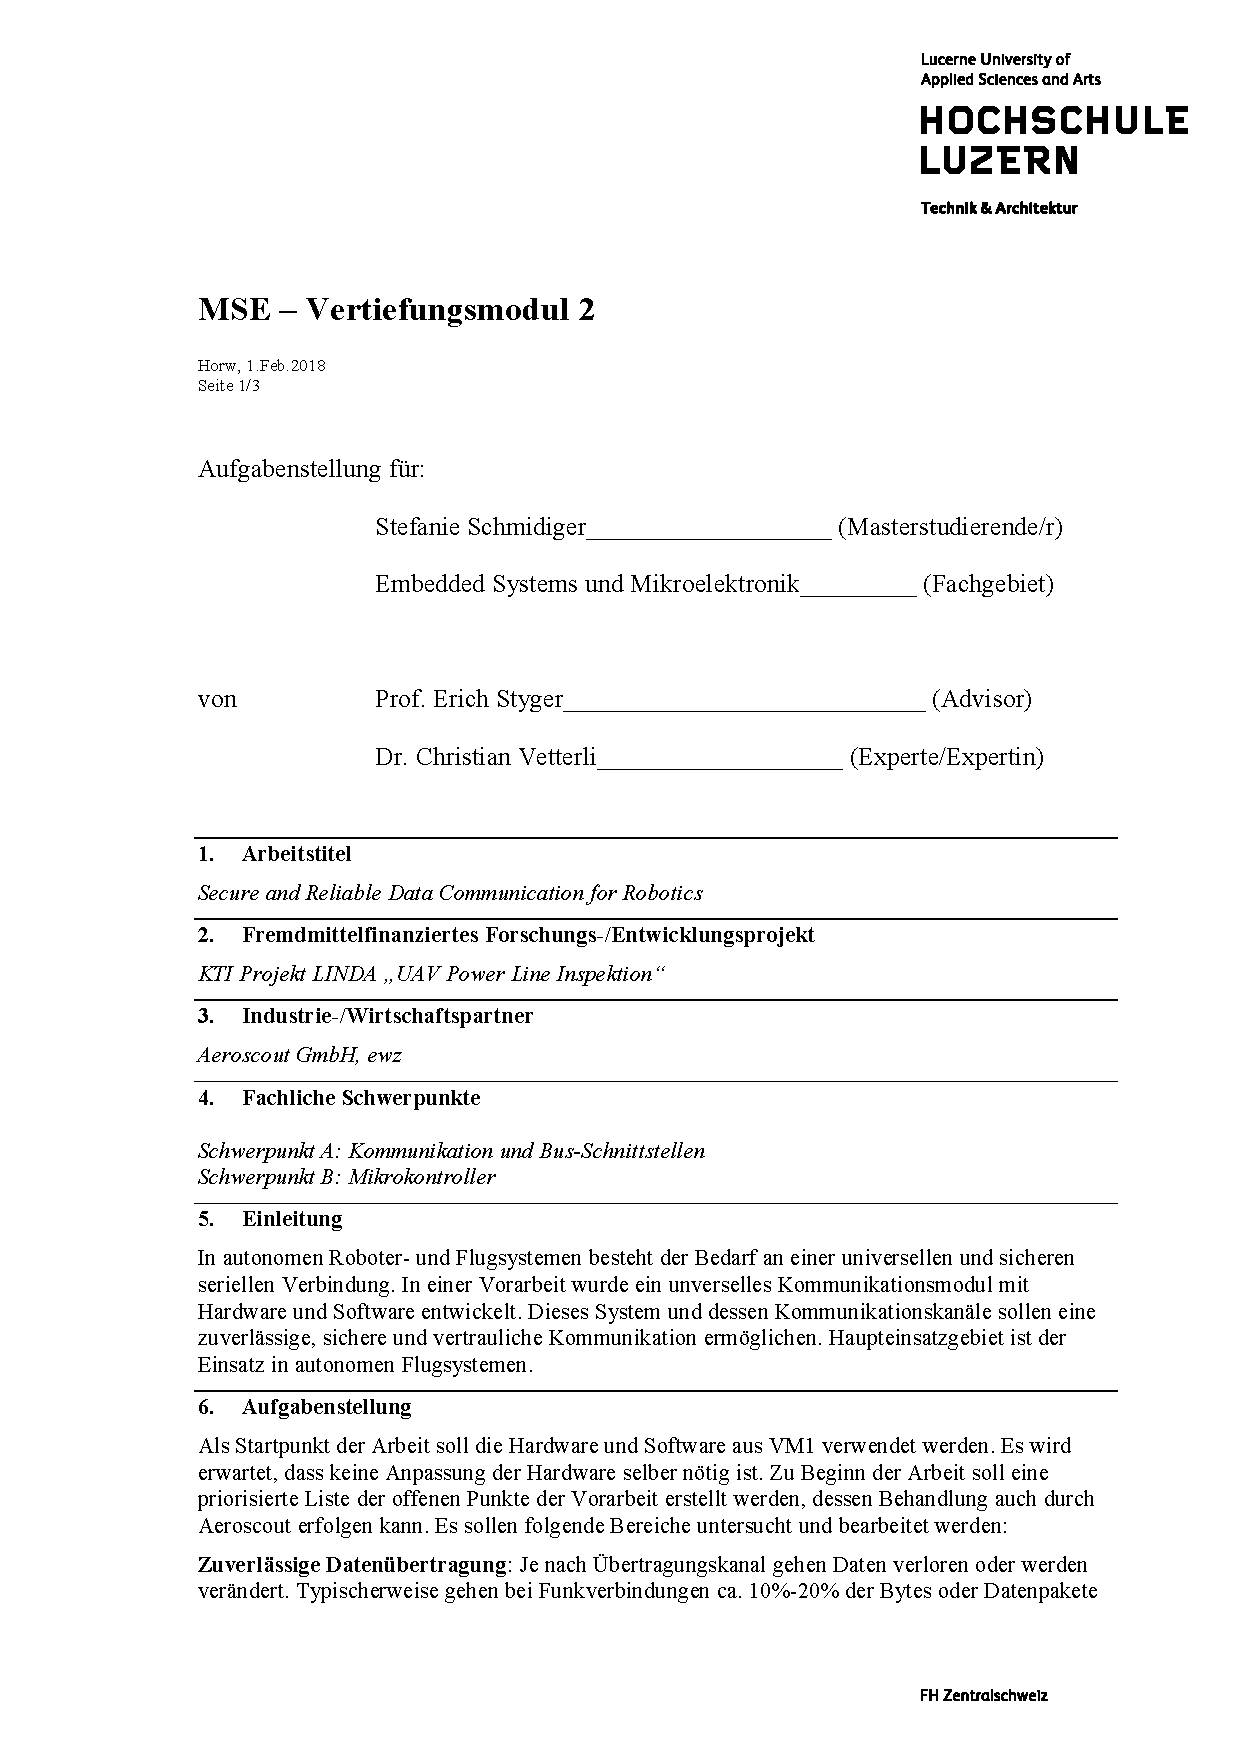
\includepdf[pages=-]{Aufgabenstellung.pdf}